\section{High-Performing Configuration Insights}
\label{sec:configurations}

\begin{figure*}[!t]
\centering
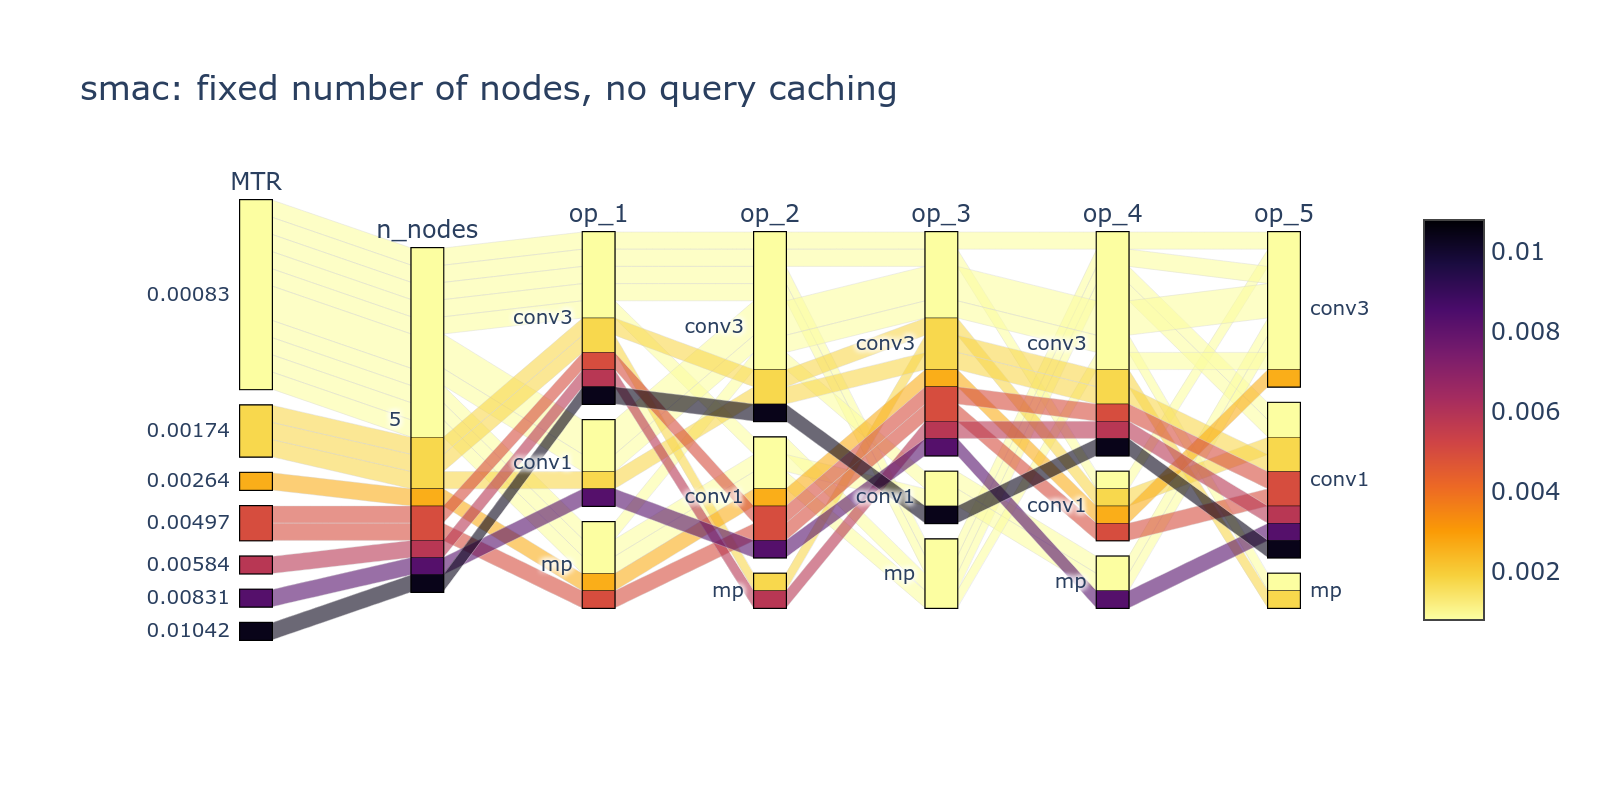
\includegraphics[width=0.47\linewidth, clip=true, trim=142px 155px 210px 170px]{imgs/parcat/smac-fnn-nc.png}
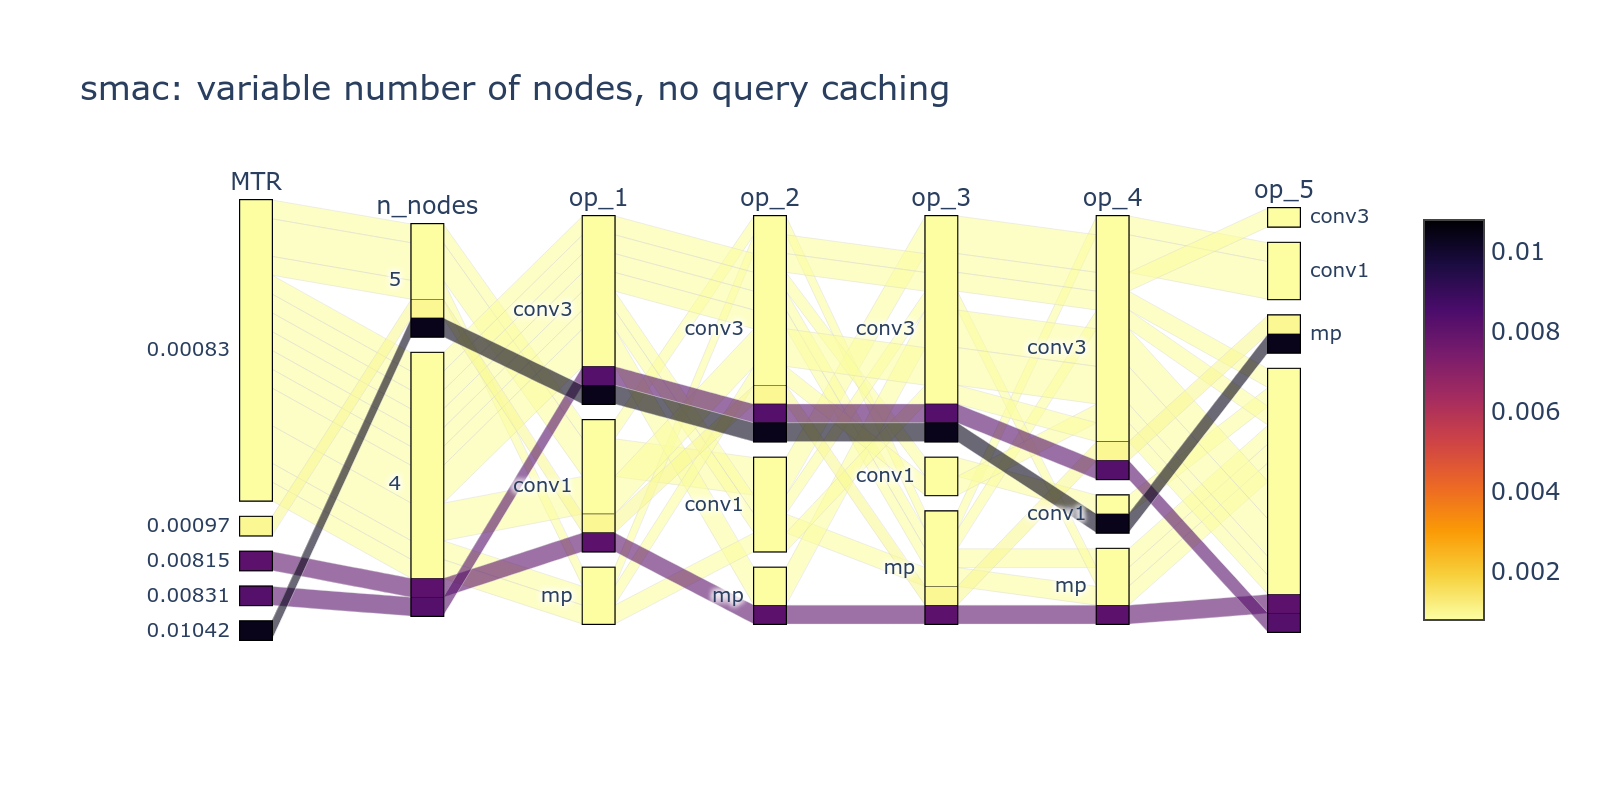
\includegraphics[width=0.51\linewidth, clip=true, trim=142px 155px 40px 170px]{imgs/parcat/smac-vnn-nc.png}
\caption{Parallel categories plots of the 20 architectures selected by SMAC with fixed (left) and variable (right) number of nodes.}
\label{fig:pc-smac}
\end{figure*}

In this section, we analyze the final configurations and thus, the architectures selected by the different NAS techniques. For this purpose, we study the configurations obtained in each run of the algorithms. Figure~\ref{fig:pc-smac} shows parallel categories plots for SMAC. For clarity, only NAS hyperpameters related to the node label list are given~(\textit{op$_1$}-\textit{op$_5$}).
% corresponding to each vertex of the DAG model, i.e. each layer of the selected neural network, for legibility's sake. 
The possible values for these parameters are \textit{conv3} ($3 \times 3$ convolution), \textit{conv1} ($1 \times 1$ convolution), \textit{mp} ($3 \times 3$ max-pooling), or empty in the case of the variable-sized approach. 
Since topology is defined by the adjacency matrix, no layer order or architecture size should be assumed.
Color scaling reflects the mean test regret, which we additionally depict as a discretized variable in the left-most column of the plot. Though conclusions in this section are drawn from all plots analyzed, the remaining ones 
%they are not all included here for brevity
% due to size restrictions, 
are given as supplementary material for brevity.

In line with the layer type performance effects reported in \nasbench, \textit{conv3} is the most frequently selected node value. This was especially true for \irace, particularly in the fixed-size approach. In fact, several of the high-performing configurations 
% across the board 
seem to use only \textit{conv3} nodes, with no \textit{conv1} nor pooling layers. This is surprising, as manual design would certainly include them. We believe that these results reflect the design for accuracy adopted in \nasbench. In particular, one of the most significant benefits from pooling is reducing training time. Yet, architectures are generally evaluated only as to their accuracy. Though it would be possible to assess some level of trade-off between architecture accuracy and total training time, we have followed the original setup from \nasbench where this is not considered. We remark, though, that this can lead to the selection of extremely costly architectures, such as the \textit{conv3}-based mentioned previously.
%which use only $3 \times 3$ convolutions.

Regarding caching, all algorithms have a hard time finding good configurations using this approach. This is a further indication of the usefulness of variability in this benchmark from a final-quality perspective. On the other hand, adopting a variable number of nodes can be beneficial, as is the case for SMAC. Yet, we remark that the architectures given in Fig.~\ref{fig:pc-smac} may present less than $n_\text{nodes}$ nodes due to their topology, which is not shown here. 
%Yet, we remark that the architectures given in Fig.~\ref{fig:pc-smac}~(left) may present less than five nodes due to their topology, which is not shown here. 
%This is also true for Fig.~\ref{fig:pc-smac}~(right), even if some architectures differ as to the NAS hyperparameter $n_\text{nodes}$. 
% the right-most a sepathat the variable approach allows SMAC to more easily find optimal configurations, which often have fewer than 5 nodes. This is not exclusive to SMAC, with other algorithms having their best configurations in the variable approach with 4 or 3 nodes,
Finally, we note that RE finds a top-performing configuration containing a single $1 \times 1$ convolution layer. We remark that this is possible due to the scalable architecture approach discussed in Section~\ref{sec:background}.

% \begin{figure*}[!t]
% \centering
% 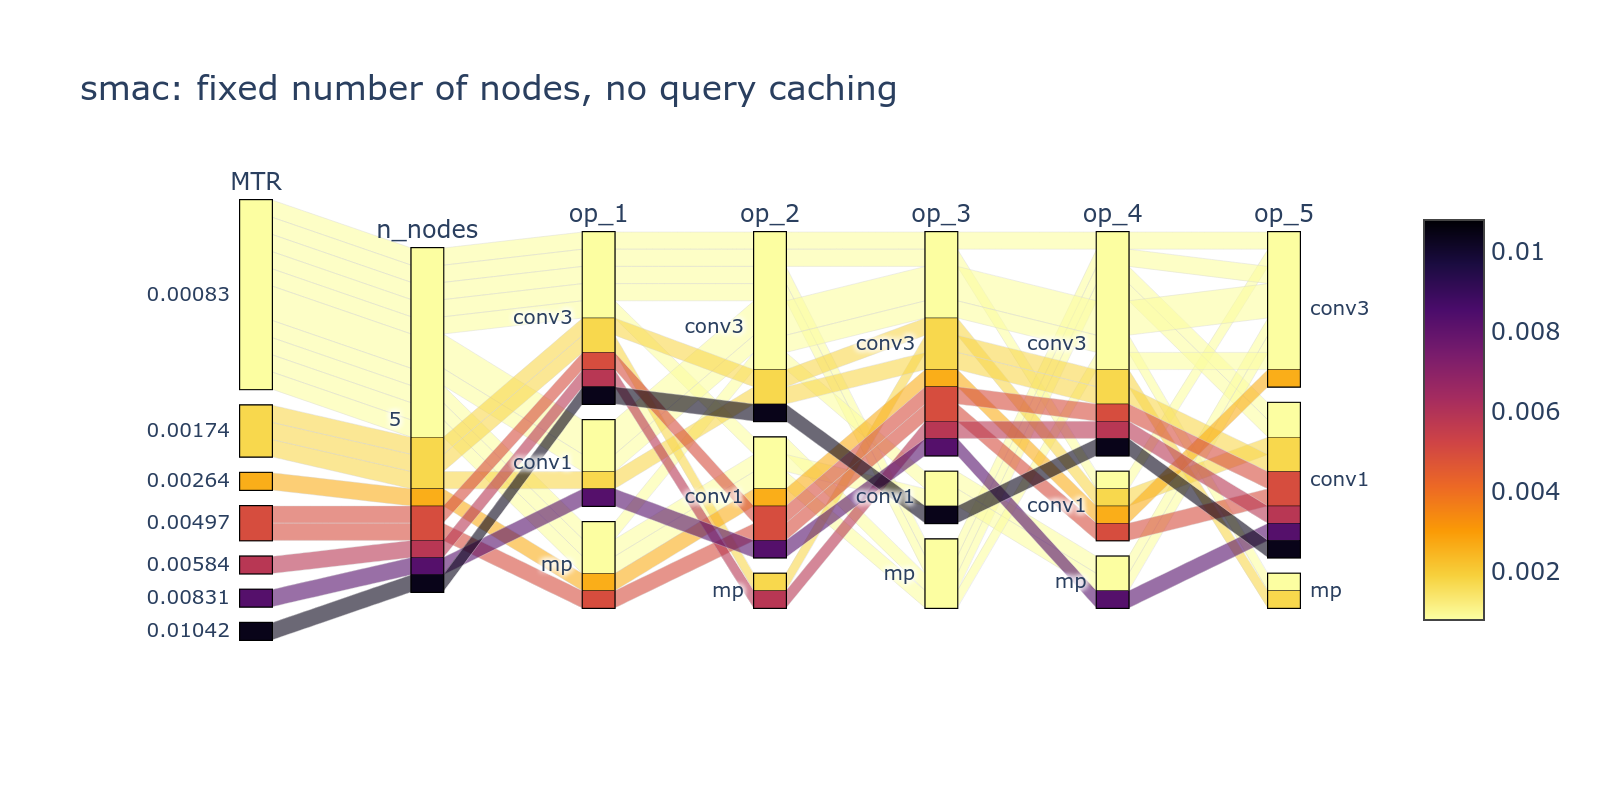
\includegraphics[width=0.47\linewidth, clip=true, trim=140px 150px 40px 150px]{imgs/parcat/smac-fnn-nc.png}
% 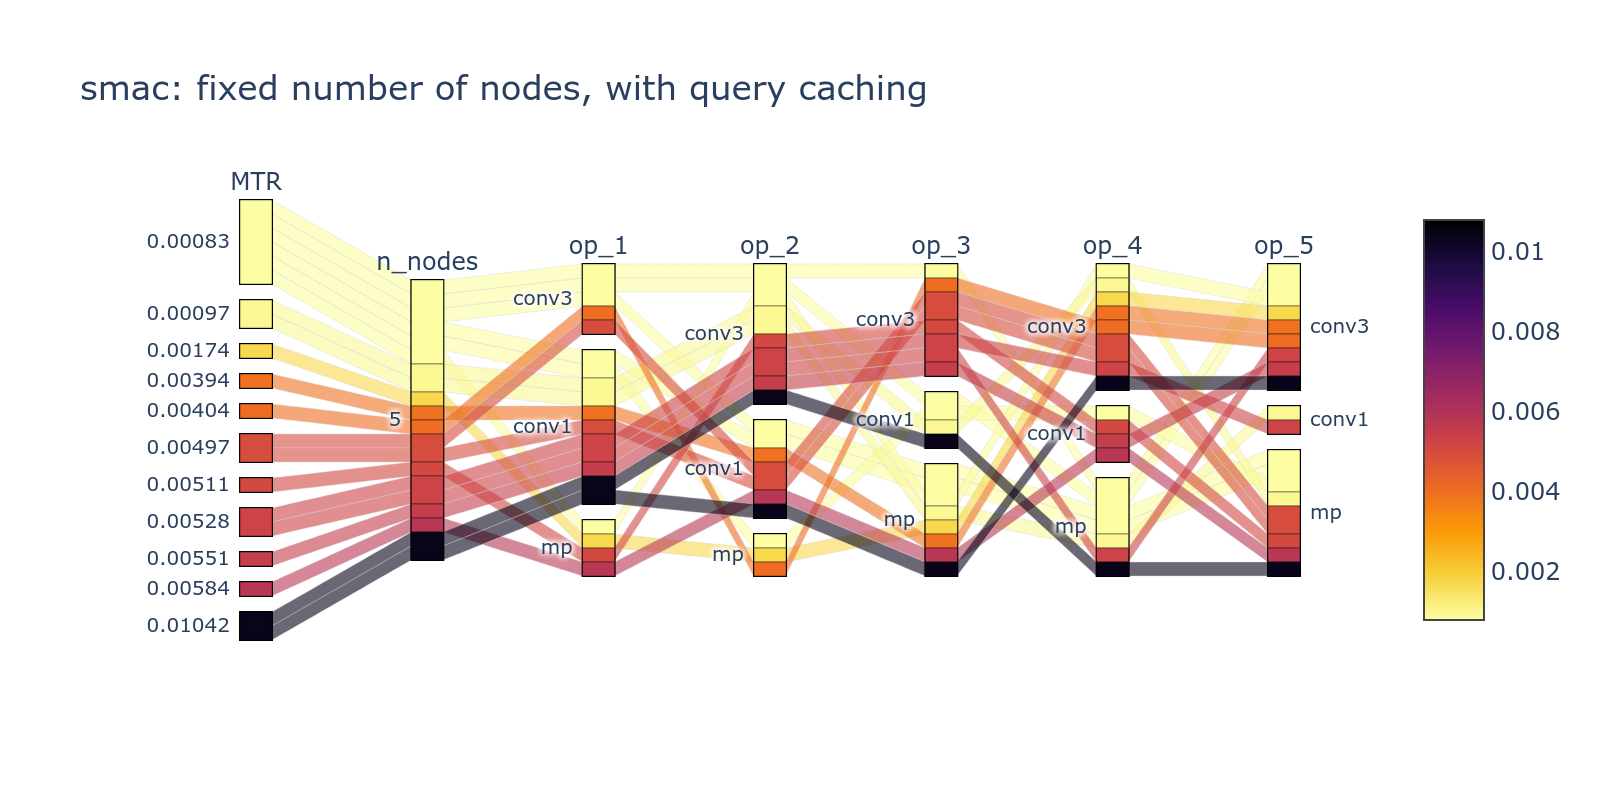
\includegraphics[width=0.47\linewidth, clip=true, trim=140px 150px 40px 150px]{imgs/parcat/smac-fnn.png}
% 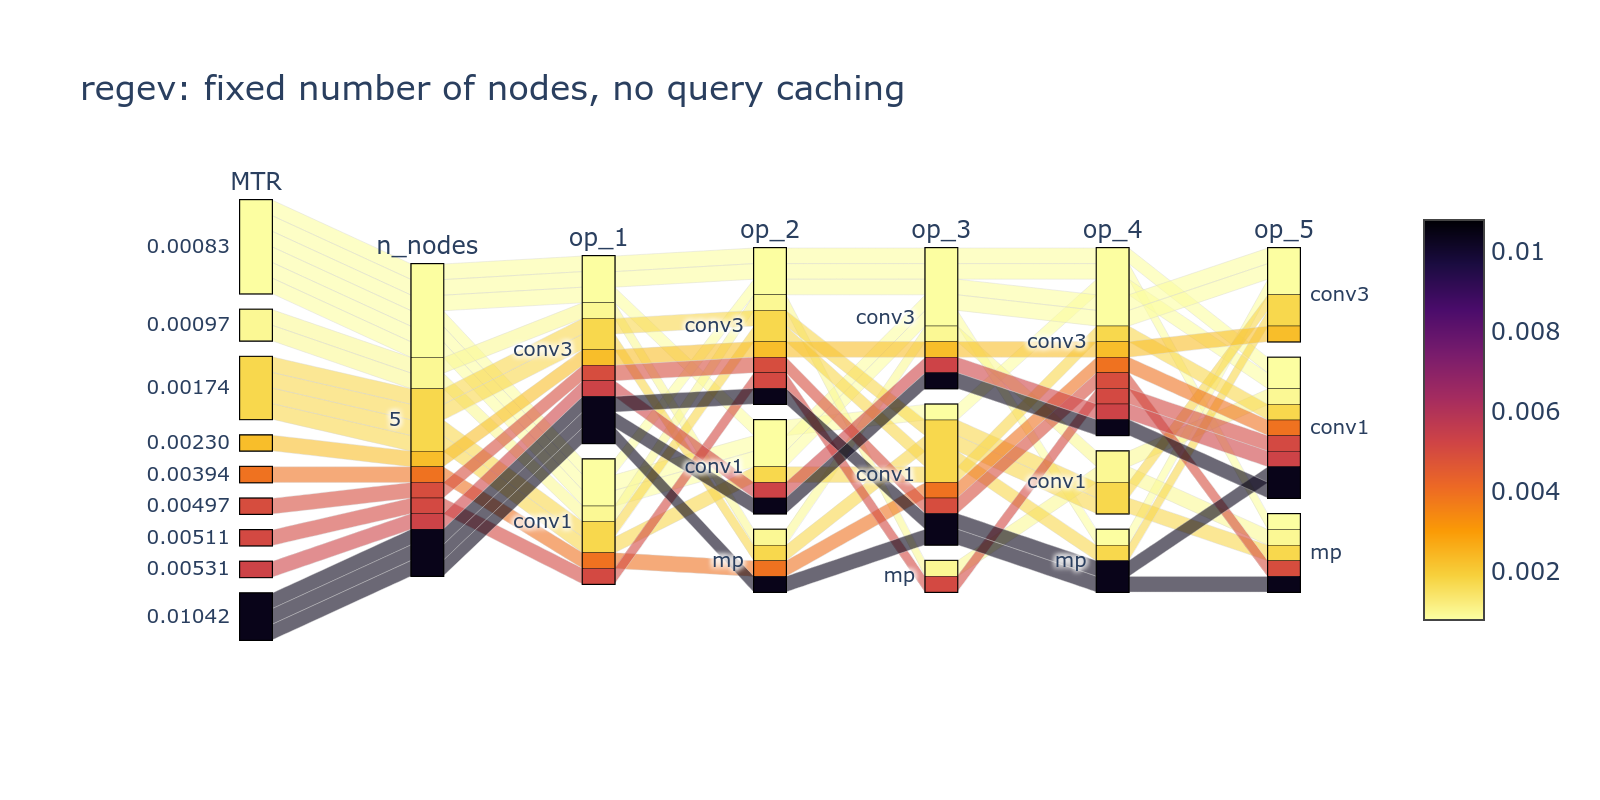
\includegraphics[width=0.47\linewidth, clip=true, trim=140px 150px 40px 150px]{imgs/parcat/re-fnn-nc.png}
% 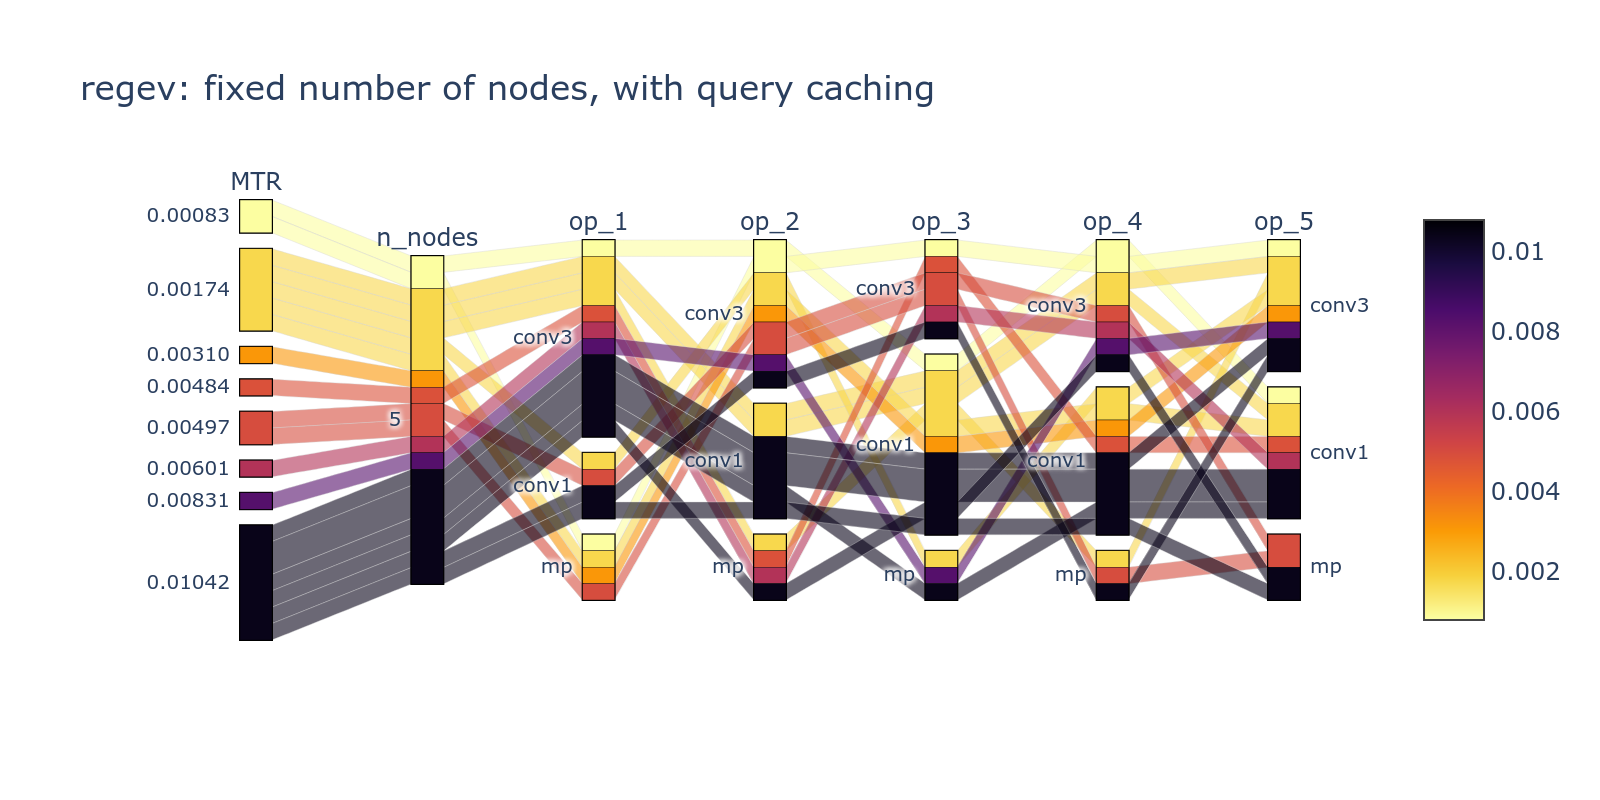
\includegraphics[width=0.47\linewidth, clip=true, trim=140px 150px 40px 150px]{imgs/parcat/re-fnn.png}
% 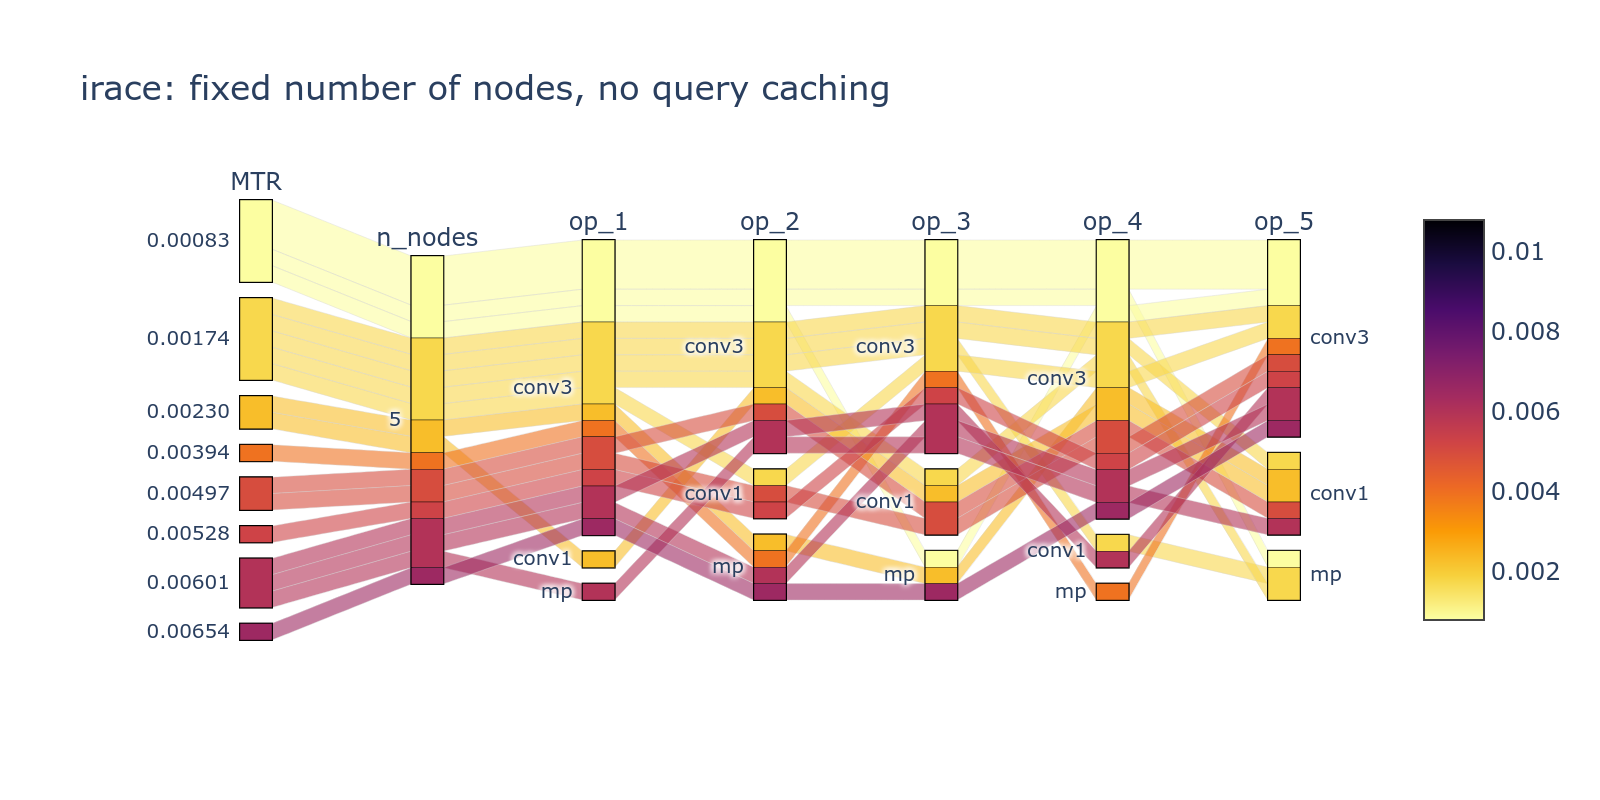
\includegraphics[width=0.47\linewidth, clip=true, trim=140px 150px 40px 150px]{imgs/parcat/irace-fnn-nc.png}
% 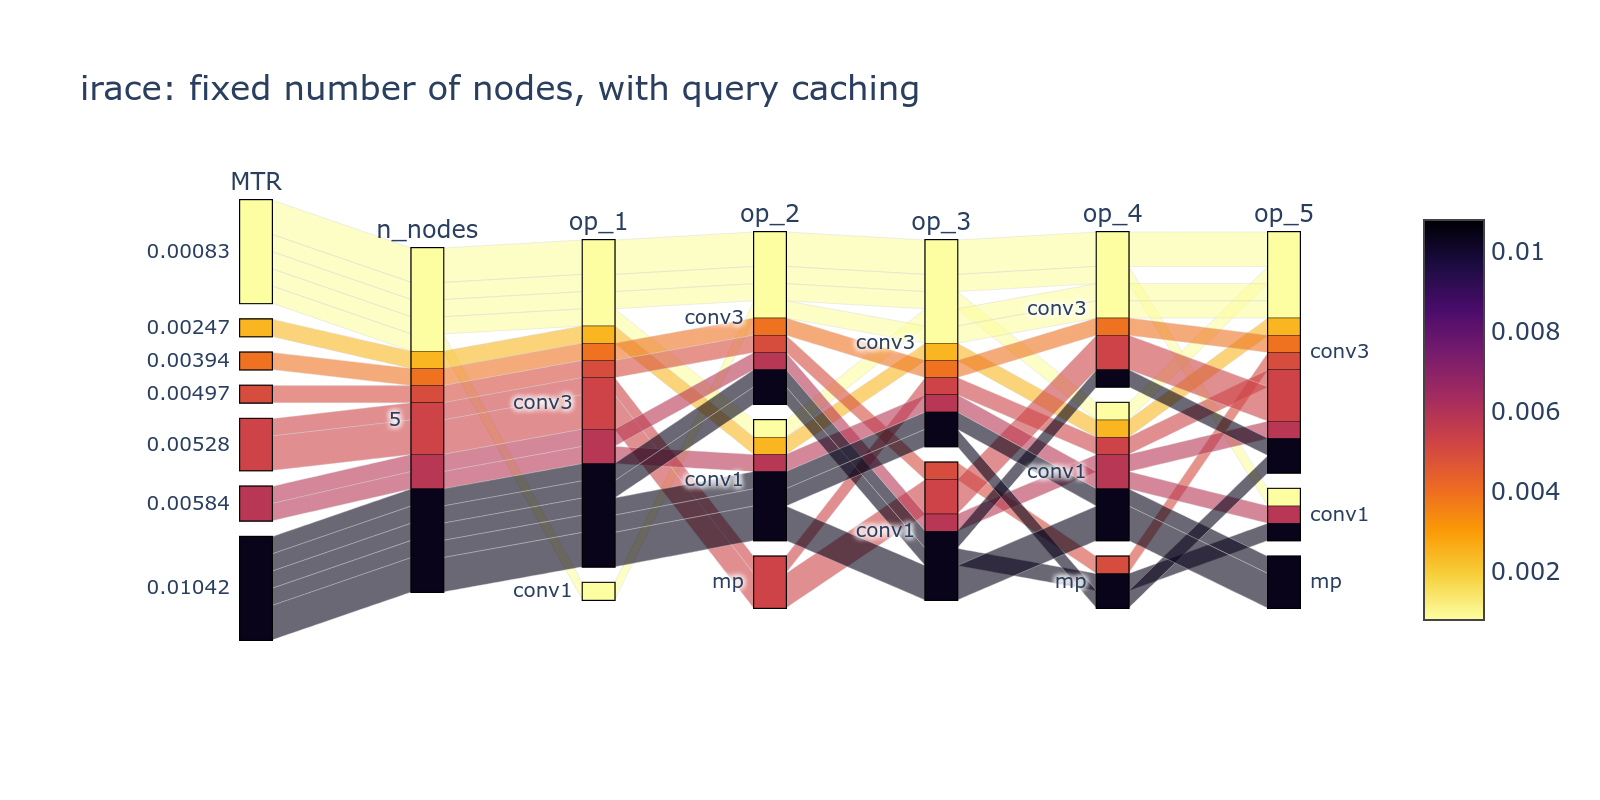
\includegraphics[width=0.47\linewidth, clip=true, trim=140px 150px 40px 150px]{imgs/parcat/irace-fnn.png}
% \caption{Parallel categories plots of the 20 architectures selected by SMAC (top), RE (middle), and \irace (bottom) with fixed number of nodes, no caching (left), caching (right).}
% \label{fig:cf-comp}
% \end{figure*}


% \begin{figure*}[!h]
% \centering
% 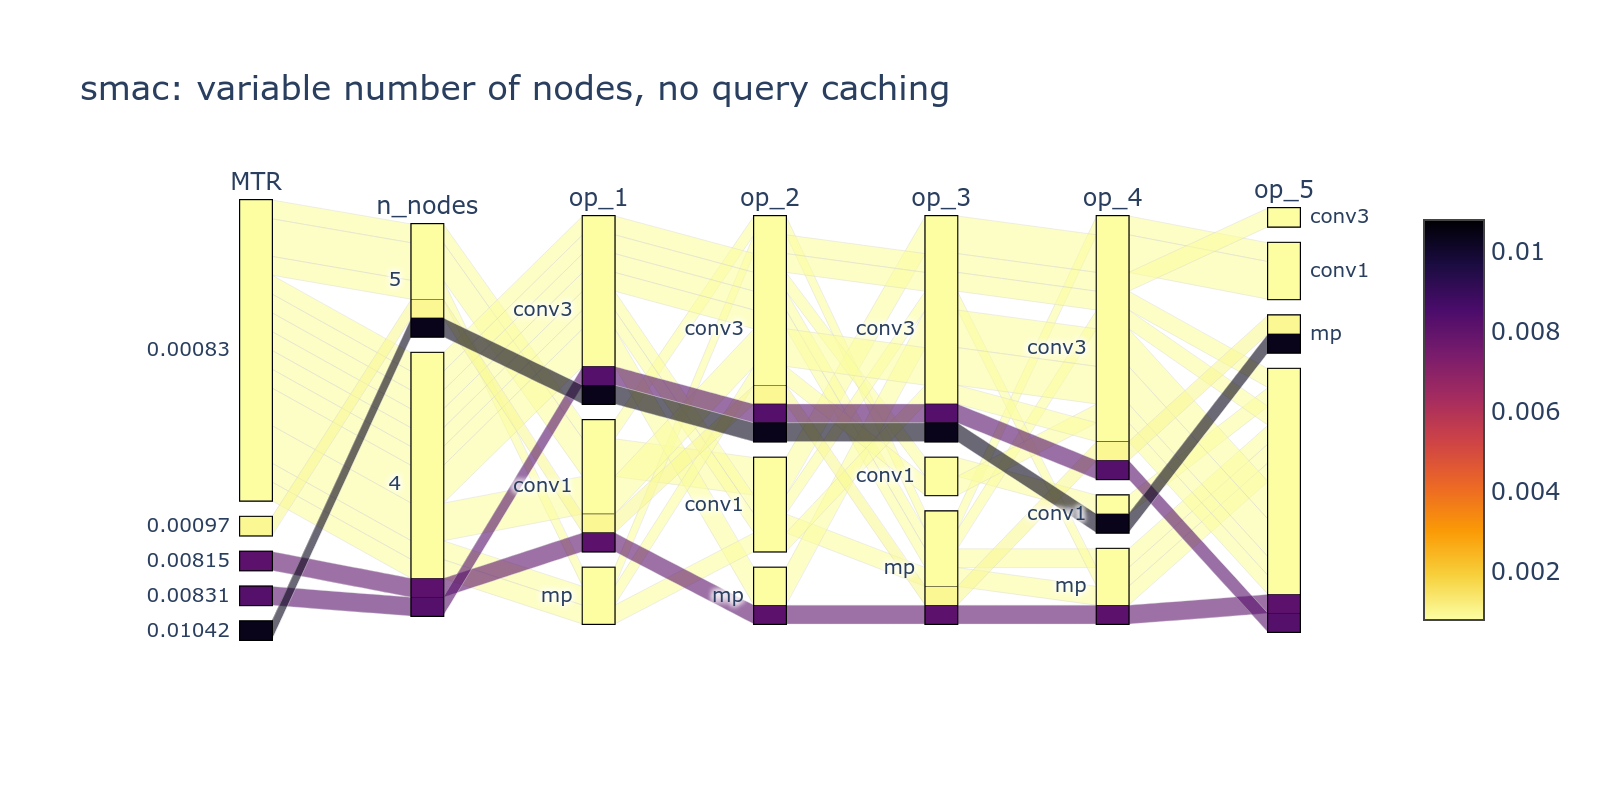
\includegraphics[width=0.47\linewidth, clip=true, trim=140px 150px 40px 150px]{imgs/parcat/smac-vnn-nc.png}
% 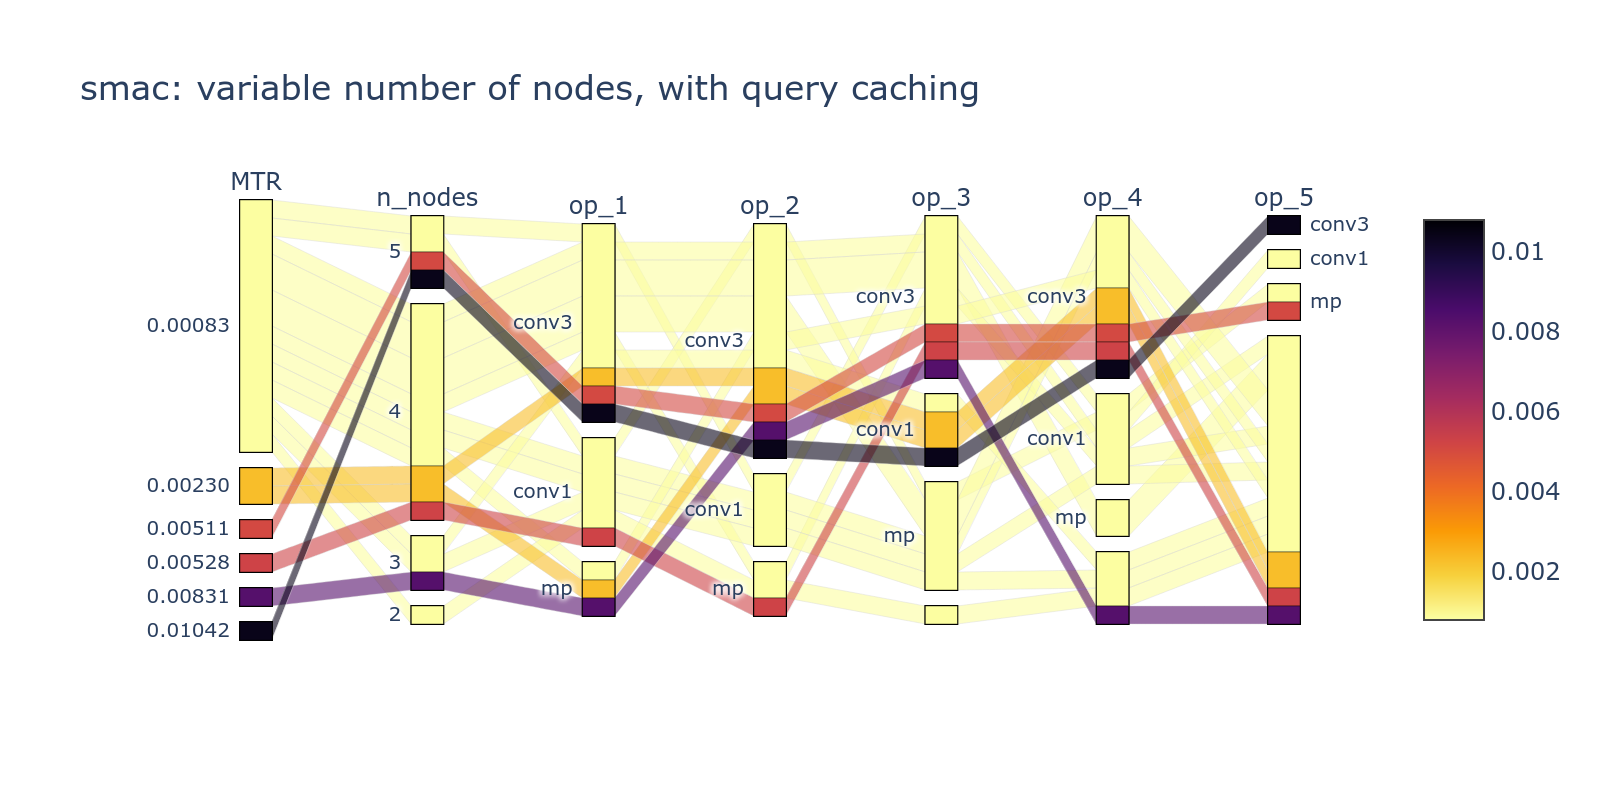
\includegraphics[width=0.47\linewidth, clip=true, trim=140px 150px 40px 150px]{imgs/parcat/smac-vnn.png}
% 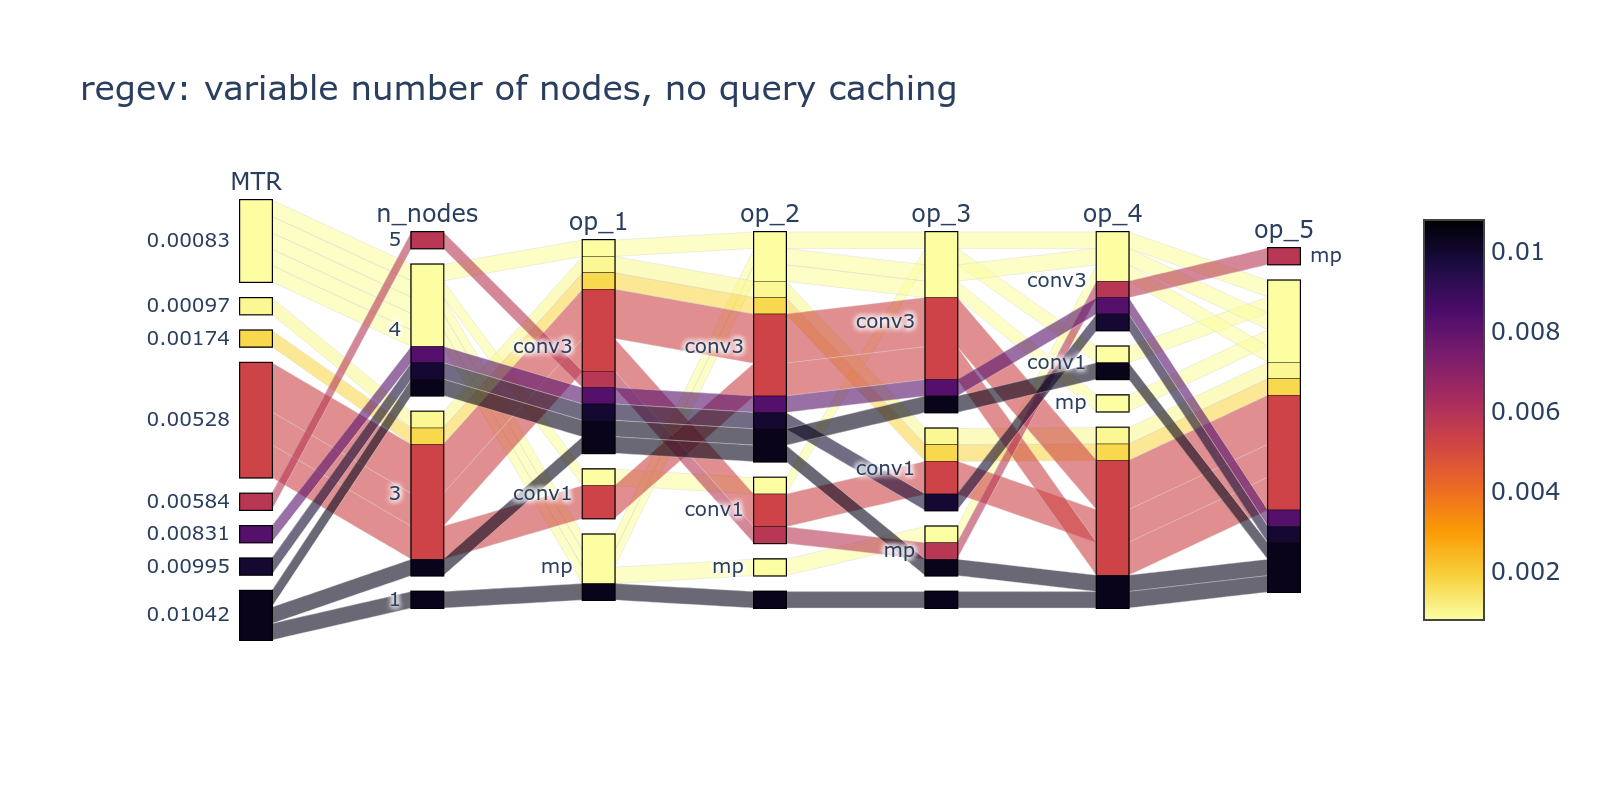
\includegraphics[width=0.47\linewidth, clip=true, trim=140px 150px 40px 150px]{imgs/parcat/re-vnn-nc.png}
% 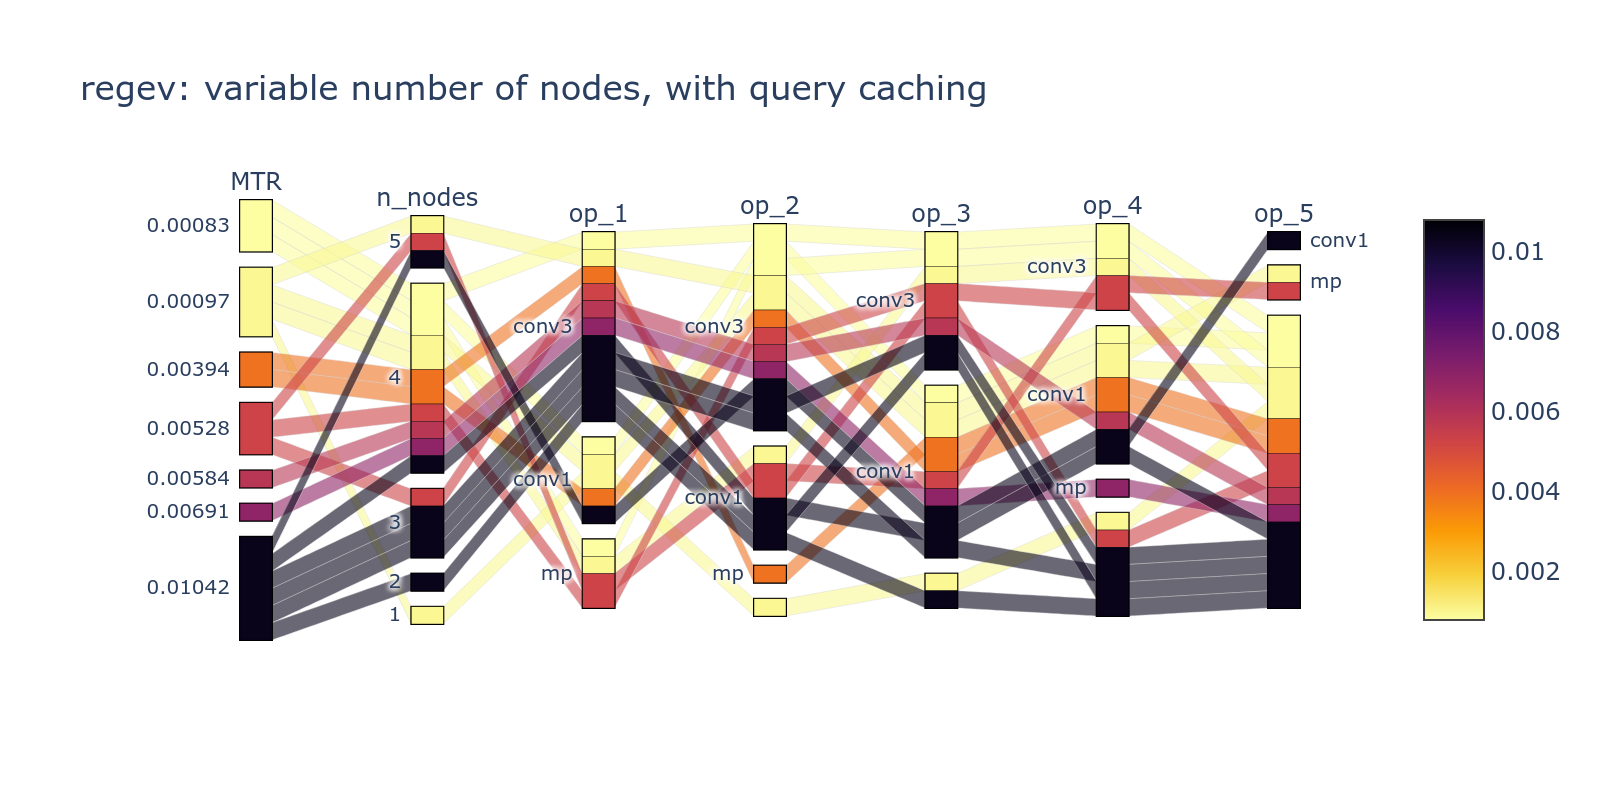
\includegraphics[width=0.47\linewidth, clip=true, trim=140px 150px 40px 150px]{imgs/parcat/re-vnn.png}
% 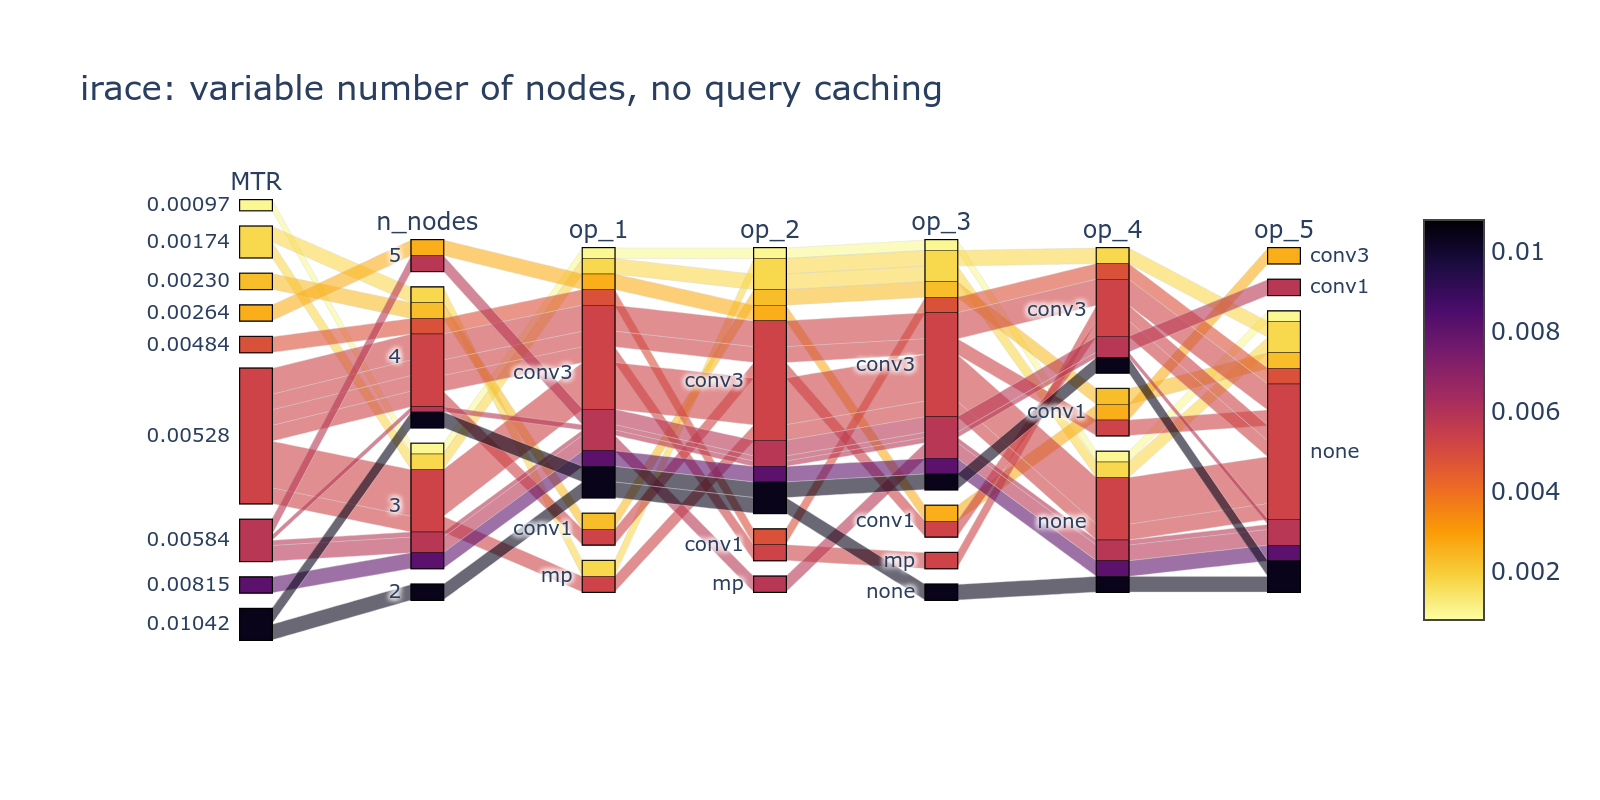
\includegraphics[width=0.47\linewidth, clip=true, trim=140px 150px 40px 150px]{imgs/parcat/irace-vnn-nc.png}
% 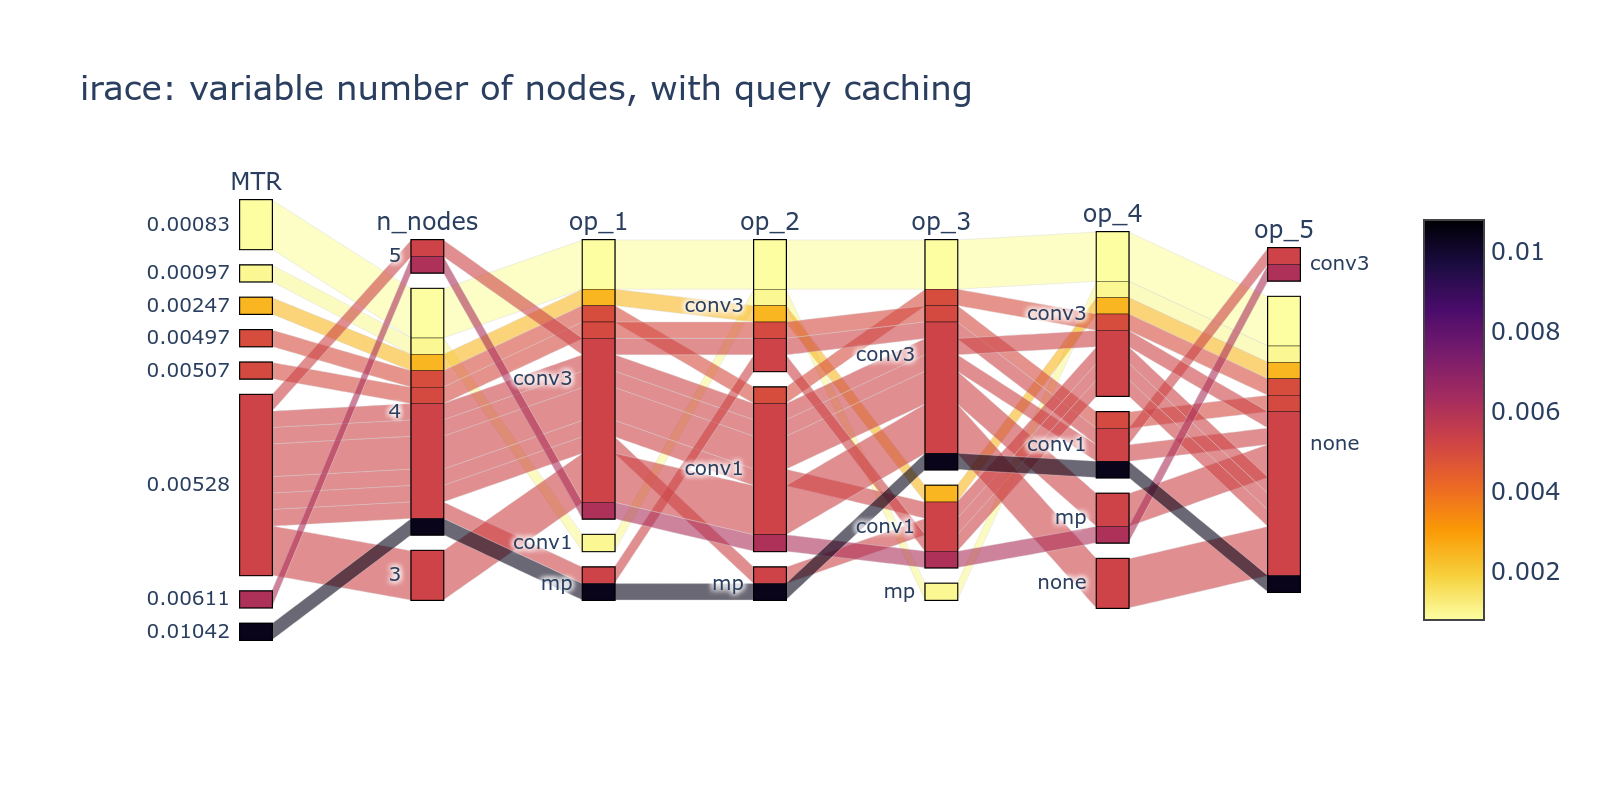
\includegraphics[width=0.47\linewidth, clip=true, trim=140px 150px 40px 150px]{imgs/parcat/irace-vnn.png}
% \caption{Parallel categories plots of the 20 architectures selected by SMAC (top) RE (middle) and \irace (bottom) with variable number of nodes, no caching (left), caching (right).}
% \label{fig:cv-co}
% \end{figure*}
